% 
% PhD Project Protocol
% Maxime Lavigne
%
\documentclass[12pt]{memoir}
\usepackage[utf8]{inputenc}
\usepackage[letterpaper, margin=2cm]{geometry}
\usepackage{hyperref}
\usepackage{lipsum}
\usepackage{graphicx}
\usepackage{atbegshi}

% Default, Single Space equals 6 lines per inch exactly.
%\chapterstyle{bringhurst} % -- the real good one
%bringhurst
%culver
%komalike
\chapterstyle{komalike}

\renewcommand{\clearforchapter}{}

\renewcommand{\section}[1]{%
  \refstepcounter{section}%
  \addcontentsline{toc}{section}{\thesection \quad #1}%
  \vspace{0.25cm}
  \textbf{\large\thesection.}%
  \space\nolinebreak \large\textbf{#1}\normalsize \quad}

\begin{document}

\AtBeginShipoutNext{\AtBeginShipoutNext{\AtBeginShipoutDiscard}}
\begin{titlingpage}

\begin{minipage}[c]{0.23\textwidth}
\raggedright 

\includegraphics[width=0.75\linewidth]{coa.jpg}
\end{minipage}%
\vrule width 2pt
\begin{minipage}[c]{0.73\textwidth}
	\centering
	
	\vspace{5cm}
	{\huge\scshape Improving your\\Clinical Practice \\ \vspace{0.5cm} for the Game's Own Sake}
	
	\vspace{2cm}
	{\Large\bfseries Thesis Protocol\par}
	
	\vspace{2cm}
	{\Large\itshape Maxime Lavigne\par}
	
	\vspace{2cm}
	supervised by\par
	Dr.~David L. \textsc{Buckeridge}
	
	\vspace{2cm}
	thesis committee\par
	Dr.~Most interesting man in the \textsc{World}\par
	Dr.~Grumpy \textsc{Cat}\par
	Dr.~Boaty \textsc{McBoatface}

	\vspace{2cm}
	{\large April 30, 2021\par}
\end{minipage}%

\end{titlingpage}

\tableofcontents
\clearpage

\chapter{Introduction and Background}
Audit and feedback (\gls{AF}) is an increasingly used quality improvement technique defined as a summary of the clinical performance of healthcare providers over a specified period of time. In essence, A\&F assesses providers' performance and compares it with established standards to then provide a summary designed to drive improvement.\cite{ivers2012audit}

There are multiple reasons why some institutions choose to use A\&F. For example, it is known that unintended and inappropriate variation in care are common, and that clinicians are relatively poor at self-assessment.\cite{davis2006accuracy} Additionally, A\&F is known to be a scalable and relatively inexpensive strategy to promote the uptake of best practices found in high-performing health systems.\cite{baker2015creating}. The added attention A\&F receives is encouraging as its improvements, even if small, could result in clinically meaningful and cost effective changes in processes and outcomes.\cite{ivers2018using}

Yet, designing effective A\&F remains difficult. The latest Cochrane reiterated that "[A\&F] will continue to be an unreliable approach to quality improvement until we learn how and when it works best."\cite{foy2005we} This is why the literature explores myriad aspects of its implementation, how it measures care, how it communicates its findings, and through what mechanisms it operates. As theories of decision making suggest, one particularly appealing lever are the  incentives surrounding certain practices. Research on incentives in A\&F has largely been targeted at the use of extrinsic motivators be it monetary\cite{campbell2007payperf}, social\cite{ehrenfeld2014automated}, or reputational\cite{schneider1998use}. This research led to encouraging results but also presented limitations. As an example, a review of pay-for-performance showed potential short term improvement in the process of care but little to no effect effect on intermediate health outcomes.\cite{mendelson2017effects} Authors pointed out some extrinsic rewards have consistent detrimental effects on intrinsic motivations and therefore on important motivators such as accomplishment, mastery and/or self-fulfillment\cite{deci1999meta}. Often characterised as playing the game for the game's own sake.

Behavioural techniques promoting intrinsic motivators exist but their effect on A\&F are unknown. Prior exploration of effective goal setting theory and self-determination theory suggest it could have a clear and beneficial impact on A\&F. Especially through the use of interactive and low-latency summaries such as those used in electronic A\&F. Gamification was shown to positively impact two important factors of an ongoing feedback system; engagement and enjoyment.\cite{hamari2014does}

\chapter{Evaluation}
The aim of this research project is to study the effect of gamification on electronic audit and feedback (e-A\&F) systems. Principally, this will require us to answer four questions:

\begin{itemize}
    \item What targets and measures are most suitable for an e-A\&F intervention, at the CHUM, in cardiology, at this time.
    \item What is the effect of gamification on the adoption of, engagement with, and retention of users of e-A\&F systems
    \item What is the effect of gamification on 
    How does it affect how effective is the base e-A\&F intervention.
    \item How is gamification perceived by the users (and what is this perception's effect)?
    \item (not marketable) How can e-A\&F be designed to offer a gamified experience consistent with the A\&F goals?
\end{itemize}

The central hypothesis of the proposed research is gamification will be an effective and well accepted way of increasing the adoption and engagement of e-A\&F as compared to a traditionally designed system, in medical doctors and trainees. This hypothesis was formulated based on the existing gamification literature and overlaps between the mechanisms of gamification and behaviour change theories. This study protocol will describe how the proposed research is to be conducted, and to ensure the safety of the study participants along with the integrity of the data collected.

\chapter{Methods}
This proposed project will be conducted over 24 months and will include three studies: (1) a descriptive analysis of retrospective data, (2) a laboratory based usability study, and (3) a randomized control trial.

 The first objective is needed to design both the control and experimental interventions and ensure they work with local data. Objective 2 will ensure that both interventions are usable and free from major bugs or obvious unintended effects. It will also be used to foresee any deployment issue with the hospital. Finally, objective 3 addresses the overall hypothesis, the effect of gamification on e-A\&F systems.

\begin{figure}[h]
    \centering
    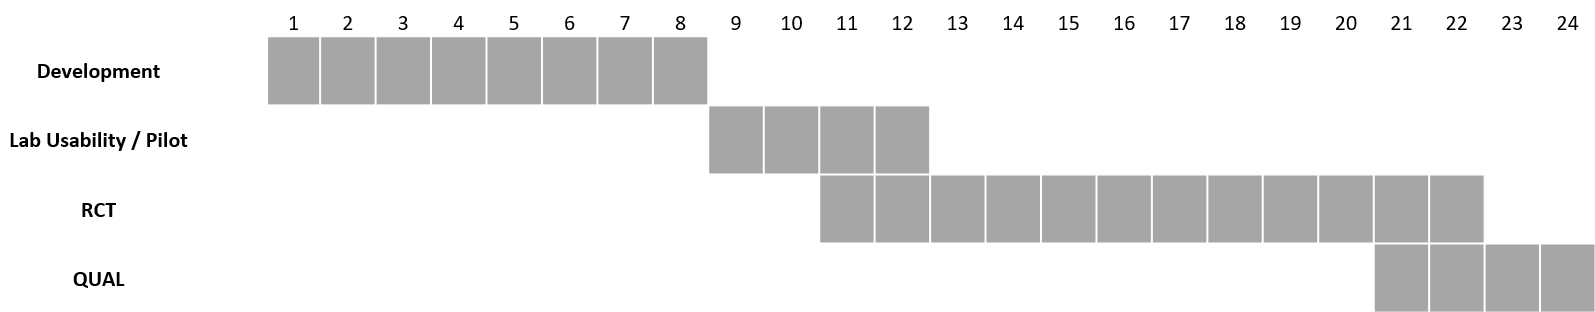
\includegraphics[width=\textwidth]{img/timeline-overall.PNG}
    \caption{Research Project, Timeline in months}
    \label{fig:timeline}
\end{figure}

\section{Data Source and Characteristics}

\begin{wrapfigure}{r}{10cm}
  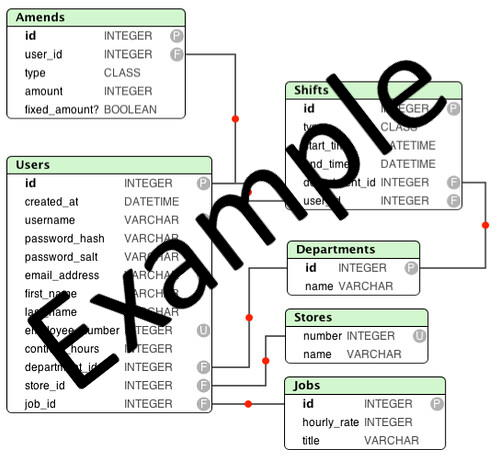
\includegraphics[width=\linewidth]{img/example_erd1.jpg}
  \caption{Entities and their relationship in the data}
  \label{fig:entity-relationship-diagram}
\end{wrapfigure}

The section discusses two distinct data needs. What is used for research and what is used in the interventions. The data for research is denominalized and seen by the research team, the data for the intervention is nominalized and only seen by the physician who undertook the care of the patient mentioned.

Patient and physician data will come from an existing system at the MUHC called the "data warehouse" (DW). A data warehouse is an enterprise data aggregation system which facilitates its collection, analysis, and reporting. The MUHC DW is already in place and contains a wide range of data relating to most aspects of in-hospital care.

This project will use two datasets coming from the same source. A first, broader and denominalized, data request will be made for the purpose of finding targets in objective one and two. This request will be placed to the research pipeline of the data warehouse. Here, the identity of both the patient or provider is of little interest as long as they have unique IDs. A second, precise, targeted, and nominalized data request will be made for the purpose of conducting the RCT. During this phase, I need to be able to have the right provider see the right feedback, but these providers also need to be able to see which patient might be in need of additional actions.

Additional data will be collected on the physician's use of e-A\&F. This data will be linked to anonymous IDs.

All nominalized data will be kept in a remote secure server in the MUHC data center. Feedback will also be created by the systems on this server. Anonymous data will be kept on a secure password protected computer, where the data analysis will also take place. All nominalized data will be removed as soon as the trial is over, while summary description of the anonymous data will be published along with the relevant research articles.

\chapter{Objective 1: Exploration of Metrics}
% Develop a set of quality indicators for e-A&F
Audit and feedback is first and foremost a way to generate new insights and inform future actions in clinical care. For this reason, the design and implementation of measurement is of critical importance to the creation of effective A\&F. The WHO describes performance measurement as a process which "seeks to monitor evaluate and communicate the extent to which various aspects of the health system meet their key objectives."\cite{smith2009performance} However, not all quality measures are created equal and the creation of suitable and successful metrics is not simple. Current evidence shows that quality measures should be aligned within an organizational context, relevant to its actors, attributable to specific individuals, feasible, accurate, and reliable.\cite{polanczyk2019quality}

For this reason, my first objective is to "develop a set of quality indicators for e-A\&F to assess and improve the appropriateness of heart failure management in adult patients at the MUHC." This set of indicators will then be used in objective 2 and 3 as it will impact (1) data collection, (2) feedback design, and (3) evaluation of the intervention.

\section{Research Design}
I propose an exploratory quantitative analysis of quality measures for heart failure at the MUHC. This study will use two years of retrospective secondary operational data to compare candidate quality measures. Data will be extracted by selecting admitted patients with ICD codes \footnote{From AHA's, Get with the Guidelines\textcopyright - Heart Failure} for heart failure along with the physicians who interacted with them. In order to match the future objective and limit the unnecessary risk to patients, data will be limited to adult patients at the MUHC.

\todo[inline]{Add information here on how many patients/doctors, we approximate this means based on Madjda numbers.}
\todo[inline]{How to justify 2 years (of HF patients, perc. complet in lit) }

Descriptive statistics will be used to provide a tabular overview of the stratified and unstratified measures, their completeness, along with a visual presentation of trends. The stratified exploration will explore the influence of basic patient demographic factors, of their cardiovascular risk, and of physician characteristics. 

\section{Evaluation Criteria}
\begin{itemize}
    \item Campbell's Prerequisites for quality measures (Acceptability, Feasibility, Reliability, Sensitivity, and Predictive Validity) \cite{campbell2002research}
    \item Key considerations when addressing causality and attribution bias (attribution, confounding, and risk adjustment) \cite{terris2009attribution}
    \item Characteristics of effective A\&F (baseline performance, availability of action plan, possible frequency, and latency)\cite{ivers2012audit} % i.e. (asap considering patient load)
\end{itemize}

Baseline performance, possible frequency, latency, attribution, and feasibility will be assessed using the basic statistics mentioned above. Acceptability will be taken into account in objective 2. Sensitivity to change, predictive validity, risk adjustment, and impact of confounders will be assessed using regression modeling. Availability of action plan will be checked manually with their relevant framework.

\section{Candidate Quality Indicators}
Multiple efforts have been made between institutions and advocacy groups to define a set of evidence-based actionable indicators for heart failure.\cite{hong2006overview}\cite{fonarow2010improving} \cite{kelley2006health} At this point, newer intervention are encouraged to use existing list of candidate measures instead of going to the source material. Doing so accelerate development and contributes to the soundness of the evidence, better face/content validity, reproducibility (between institutions), and more evidence on their association with significant health outcomes.\cite{smith2009performance}

The list of candidate retained is the result of a recently compiled systematic review of quality indicators in the ICU.\cite{goldfarb2018systematic} Its set of high-quality indicators will be considered first. But, if too few indicators are meeting the evaluation criteria, more indicator will be chosen from their expended list by local HF experts.

% Quality measures on heart failure can be from four domains: structure (), process (), outcome (), and patient experience (). The choice of quality measures has an important impact on A\&F since, for example, process measures are easier to collect and quicker to influence, but outcome measures are closer to the what healthcare is about. Measures which are stated or derived from more behavioural perspective seems to work better. Finally, quality measures which already have high compliance have, by the ceiling effect, less opportunity for improvement. 

\chapter{Objective 2: Pilot Assessment}
% Lab Usability testing
\begin{itemize}
    \item Basic Usability
    \item Topics of Comments
    \item Adverse Effects?
    \item Scalability and Deployment Testing/Planning
\end{itemize}

\chapter{Objective 3: Randomized Evaluation}
% Randomized Control Trial
https://library.gv.com/how-to-choose-the-right-ux-metrics-for-your-product-5f46359ab5be

\textbf{Randomized Control Trial with Qualitative Embedded Measure}

The proposed research design is a two-arm randomized control trial of a gamified e-A\&F system compared to an adapted existing system on the clinical performance of physicians in one hospital centre of Quebec. The control system will be adapted from an existing system’s user interface to include comparable information on users’ performance.

The project can be divided in three phases. In phase 1, the clinical team and research partners will work on the content of the A\&F intervention and at the same time an initial implementation of the system is performed. In phase 2, pilot testing is done in laboratory condition to study the system’s usability, the viability of the instruments, and assess the feasibility of the in-hospital deployment. Finally, phase 3 is a 12 months period in which clinicians are recruited, randomized, and data is collected on their practice and the use of the system. This phase will also contain a qualitative embedded study investigating the subject’s perceptions of different aspects of the A\&F system such as potential unintended effects or the adequacy of the targets.

The RCT 12 months is an trade off between longer time for ecologically relevant study period for sustained used and time feasibility concerns.
Some kind of impact evaluation could have been used, but an RCT will provide results which are likely to be more comparable with the literature, and therefore more easily usable 
\begin{figure}[h]
    \centering
    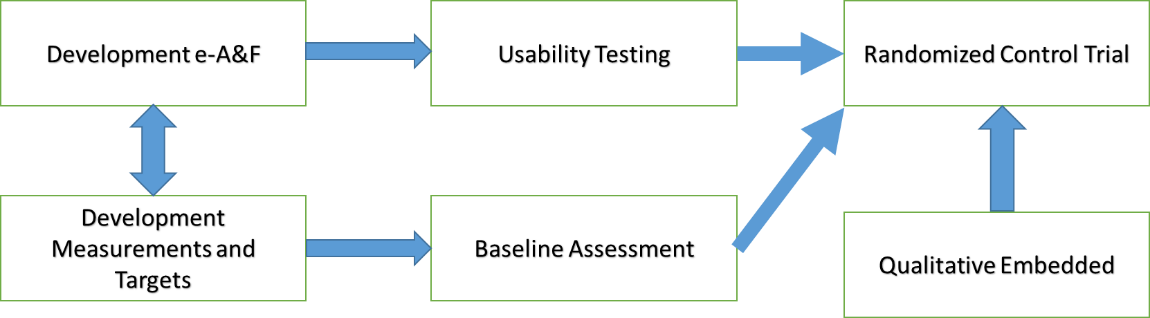
\includegraphics[width=\textwidth]{img/overall_sequence.png}
    \caption{Overall sequence, research project}
    \label{fig:ove_seq}
\end{figure}

The participants will be physicians and trainees from the participating department. Informed consent will be obtained and participants can step out at any time. Performance feedback will be confidential and personal. No clinical data will be captured specifically for this project, only secondary data will be used. The A\&F system will leverage the MUHC data warehouse to automate data collection.

\begin{figure}[h]
    \centering
    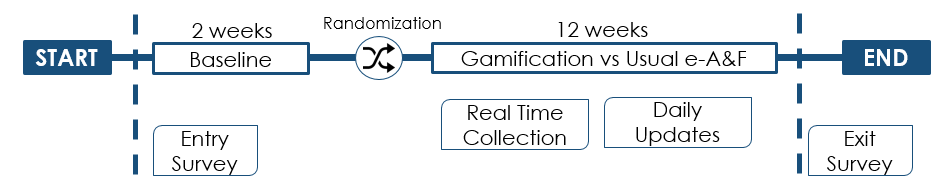
\includegraphics[width=\textwidth]{img/rct_flow.png}
    \caption{Diagram of the RCT process}
    \label{fig:rct_flow}
\end{figure}

\subsubsection{Participants}
* Attending Physicians, Residents (Cardiology, and others), Fellow

Physicians of the cardiology ward, at the MUHC Glen hospital.

Includes : Attending physicians, residents (IM and others), fellows
Eligibility : At least one month as part of the IM ward
Locations : Single Centre
Characteristics : 
Highly educated
Limited Time
Spectrum of ages
Variable IT familiarity


\subsubsection{Recruitment and Consent}
* Recruitment plans and consent process

\subsubsection{Randomization Method and Blinding}
== Randomization

Stratification levels : Attendings / Residents

Chosen randomly (by the system) after a user logs in with their user type.

Anonymous ID is created and associated with user profile in secure DB.

Randomization will likely be imbalanced on some aspects due to low Ns.


== Blinding

Blinding researchers but not participants

Participants can’t be blinded to this

Researcher can since data is collected automatically using anonymous IDs

Analysis can be blinded by not knowing which group is which.

Baseline questionnaires are taken before participants are randomized.


\subsubsection{Data Collection}
\lipsum[2]

\subsubsection{Risks and Benefits?}
Needs plan to prevent rejection, lack of trust, or perceived intrusion

\lipsum[1]

\subsubsection{Withdrawal of Subjects}

Participants can stop using their assigned system at anytime, but they won't be allowed access to the other branch. If participants either want to leave the study, or expect they won't handle case in this department anymore, an exit questionnaire will be given at that time.


\lipsum[1]

\subsubsection{Interventions}
Individual confidential Web-based portal, delivered through navigating to a specific URL on a ward computer or personal device.
No ready made public base e-A\&F to compare (and would be difficult)
Gamification is difficult to isolate (more of an emphasis then new feature)
Difficult to consider perfect fair comparison in this case, because different in many respects and no clear guidelines on what is a base e-A\&F. (specific feat. List with demo/screen will be made)
Groups will receive the same amount, and kind of implementation effort.
Support staff on hand for both solutions,  reported Severe bugs, and potential adverse effects will be fixed during trial.

\subsubsection{Measures and Outcomes}

\textbf{Entry Questionnaire}
Basic demographic questionnaire

Technology Assessment Model v3 (v1 1989, v3 2008) validated and std.
Based on Theory of Reasoned Action
Deals with Perceived Ease of Use and Perceived Usefulness
Sub. Cri. : Computer Anxiety, Comp. Playfulness, Comp. Self-Efficacy, external control.
Known confounder of IT use and effective use.

\textbf{Main Measures}
Primary
Adoption (as count of login <= 30 days)
Sustained Use (as login rates > 30 days)
Not standardized, most are marketing metrics.

Performance targets, as defined by the A\&F committee.
Likely continuous measure for 1) DM care and 2) antimicrobial use
All process measures

\textbf{Exit Questionnaire}
Something that matches our behaviour change framework?


\begin{itemize}
    \item Adoption \\ How is it measured?
    \item Engagement \\ How is it measured?
    \item Effectiveness (EMM?) \\ How is it measured?
\end{itemize}

\subsubsection{Statistical Plan}

Two arm, parallel design, individual RCT using a intention to treat (ITT) approach.

Cross-over might not be appropriate due to concerns of carryover effects.

(There will be no stop rule, due to the difficulty of finding good prior)

Bayesian sample size analysis, using priors from past study on adoption and sustained use.

Average Length Criteria to ensure for the comparison of credible intervals

Including priors on participation rates

We will used bayesian missing data technique to predict missing data on the TAMv3 and demographic baseline questionnaires.

Comparison of overlapping credible intervals for 
	counts in adoption 
	rates for sustainability
	proportions in the performance measures

Using same priors for adoption and sustain used
adjusting for any unbalanced confounders (age, sex, TAM)
Controlling for their strata

\textbf{Missing Data}
Stuff



\section{Sample Size / Precision}
Everyone?  How many is everyone.  Can we do a quick test to see howclose will this be to sufficient?  Difficulty in putting a clinical meaningfulness threshold?

\section{Ethical Considerations?} % Do I even need this?
Performance feedback is confidential, and won’ t be shared (unless required by law)
* Taking time away from patient treatment/asking for doctor's time outside of work hours?
* Informed consent will be required from all participants, but not from patients.

-- ?
* Saying something medical, possibly opposite?

\section{Research Team}
MCHI Software Development Team
	Experience in creating innovative and award winning clinical software.
	Includes skilled user support personnel and User Experience Developers.

McGill trainee / Students
	Research Assistant (or MSc. Student) and PhD students.

Clinical Contact
	Director of the Quality Assessment Unit and prior Chief of Service in IM.


\chapter{Difficulties}
A major challenge in designing this electronic audit and feedback system is, in collaboration with the clinical team, find quality improvements topics which are important for the users, have data and quality standards available, and are appropriate targets for A\&F. This also means having clinical partners which are willing to take time to participate in the governance of this project.

Designing, developing, and deploying an e-A\&F system will be time consuming and require expert knowledge in software development and information technology. However, the principal investigators as years of experience in software engineering specifically in large healthcare systems. Additionally, resources and staff from the McGill Clinical and Health Informatics research group will be available for support.

Any ongoing quality improvement effort which overlaps with this project will be a threat to the estimation of generalizable causal effects since it would confound the effect of the intervention.

Finally, since gamification is a holistic strategy which require thinking from the design process. It is first difficult to find a valid comparator, and second difficult to decompose into essential components. This is why we suggest adapting an existing system to the clinical topic chosen instead of building a synthetic comparator. Furthermore, our initial results on the whole system can then inform other teams to decompose it in a more factorial way to see which components are the most important. 

\subsubsection{Strengths and Limitations}

\begin{itemize}
    \item RCT results are comparable, easier to use along the lit, and less impacted by bias, in addition to adjusting for measured and unmeasured confounders.
    \item Lab usability made sure the system works.
    \item Team member inside the environment and known (respected)
    \item Can’t predict the effect of main outcome on patient outcome
    \item Unclear what is a clinically significant effect on adoption
    \item The same development will be used throughout the research (multiple studies for same base cost)
    \item Framework for this project will be made open source and available for future development
    \item Given the nature of the environment this is likely to be underpowered, yet multi-centre is unrealistic.
    \item Designers are evaluators, and difficult to create a valid comparator
    \item Missing richness of the experience due to RCT.
    \item Volunteer  bias likely in high performer, which are less likely to improve.
    \item Contamination likely (culture wise, and between individuals)
    \item Mechanism to combat attrition could interact with intervention.
\end{itemize}

\begin{itemize}
    \item Given the nature of the environment (few attending physicians even in large ward), this is likely to be underpowered, yet multi-centre is unrealistic. (20-10-30)
    \item Designers are evaluators (also a problem given we are creating our comparator)
    \item Missing richness of the experience due to RCT.
    \item Some residents will be part-time
    \item Volunteer bias likely in high performer, which are less likely to improve.
    \item Contamination likely (culture wise, and between individuals)
    \item Mechanism to combat attrition could interact with intervention.
\end{itemize}

\chapter{Contribution to the Literature}
In this project, three contributions will be made. Given this will be the first gamified audit and feedback system, we will be able to report on the collaborative design process and describe a process which can then be replicated elsewhere.

Second, this project will provide estimates of the effect of gamification on adoption and engagement, providing the literature with an alternative strategy to what has often been expensive reward schemes without clear benefits. Alternatively, current evidence on the effect of gamification is often provided for the lay public, this research will generate evidence about the effect of gamification on a set of highly educated professionals.

Finally, this research will provide quantitative estimates of the effect modification of gamification on the performance of the e-A\&F system. Along with it, we will provide qualitative data on the participants’ perception of the gamified system and on its impact on their motivation and intentions.

\chapter{Conclusion}
Past research on gamification showed that it works to create engagement, increase time spent, and change behaviour. Looking at the theory underpinning A\&F, it shows overlap with how gamification works and suggests it could work well. Studying gamified systems presents challenges but could lay the ground for further research to elucidate which elements or mechanism are most important for A\&F.

\chapter{Questions}
\begin{itemize}
    \item Can I distinguish between what is done by a trainees/mentor or will this always be under the mentor's name.
\end{itemize}

\begin{itemize}
    \item The written protocol should emphasize the importance of the research objective(s) and the proposed methods for addressing them.
    \item It should provide sufficient background and detail on data sources; research design, statistical analyses, and power/precision/sample size for each of the research objectives; and study limitations.
    \item The student should make clear in the protocol text the extent of his or her original contribution to the proposed research, as well as the likely format (“traditional” vs manuscript-based) of the thesis.
    \item The protocol should be limited to 10 pages (excluding references) on 8.5” X 11” paper in 12-point font and a minimum of 2 cm for all margins on each page.
    \item To permit adequate space for the methodologic aspects of the proposed research, we strongly suggest that the Background (Introduction) section of the protocol not exceed 2 of the total 10 pages.
    \item Although students may submit appendices containing tables, figures, equations, or text beyond the 10-page limit, the reviewers are not obligated to read these materials, to avoid advantaging students who submit them or disadvantaging those who do not.
    \item Thus, all key elements of the proposal should be included within the 10-page limit.
    \item The full protocol must be sent by e-mail to the course instructors, the external reviewer, and Katherine Hayden no later than 17:00 Eastern time two weeks before the defense date.
\end{itemize}

\newpage
\bibliographystyle{plain}
\bibliography{protocol.bib}

\end{document}